\chapter{Сравнителен анализ – експерименти и резултати}

Прогнозирането в мобилното приложение от страната на клиента се извършва с трислоен перцептрон. Времевия ред се разбива на двойки минало-бъдеще, които съставляват обучаващите примери. Разделението на минал и бъдещ период е условно. Практически, цялата информация е от данни в миналото. С пълзящ прозорец, условното разделяне се получава за минали стойности и стойности в бъдещия момент, спрямо условния разделител. Разполагайки с тренировъчни примери, процесът по обучението на трислойния перцептрон е свързан с търсене на тегла, водещи до минимизирането на общата грешка, която мрежата допуска. В системата са реализирани два начина за търсене на оптимални тегла – точни градиентни и евристични. Двата начина се активират на случаен принцип с равна вероятност (Листинг \ref{list0020}).

\begin{lstlisting}[caption=Превключване на алгоритмите за обучение, language=Java, basicstyle=\tiny, label=list0020]
/* Switch between gradient and evolutionry algorithm. */
if (PRNG.nextBoolean() == true) {
	/* Gradient-based optimization. */
} else {
	/* Evolutionary optimization. */
}
\end{lstlisting}

Ефективността на двата начина за оптимизиране на теглата се подлага на изследване, като алгоритмите се изолират да работят самостоятелно, извън общата работа на системата. 

\section{Точни числени алгоритми}

Encog Machine Learning Framework поддържа множество алгоритми за обучение на изкуствени невронни мрежи, като от тях са избрани пет точни числени методи (Листинг \ref{list0021}).

\begin{lstlisting}[caption=Набор от точни числени методи, language=Java, basicstyle=\tiny, label=list0021]
/* Selection of gradient-based training. */
Propagation[] propagations = {
	new Backpropagation((BasicNetwork) network.clone(), examples),
	new ResilientPropagation((BasicNetwork) network.clone(), examples),
	new QuickPropagation((BasicNetwork) network.clone(), examples),
	new ScaledConjugateGradient((BasicNetwork) network.clone(), examples),
	new ManhattanPropagation((BasicNetwork) network.clone(), examples, PRNG.nextDouble())
};
\end{lstlisting}

Класът Backpropagation реализира традиционният алгоритъм за обратно разпространение на грешката, който разчита на частни производни. При алгоритъма за обратно разпространение на грешката съществува проблем с магнитута на на производните, когато те дават твърде големи или твърде малки стойности. Втори недостатък на алгоритъма за обратно разпространение на грешката е, че параметърът са научаване (learning rate) е една единствена стойност за цялата мрежа. 

Класът ResilientPropagation реализира подобрение на алгоритъма за обратно разпространение на грешката, като въвежда коефициент за обновление (update value) на всяка връзка между два неврона. Значително предимство е, че конкретните стойности за коефициента на обновление се определят автоматично и не е нужна човешка намеса. Това е водеща разлика от класическия алгоритъм за обратно разпространение на грешката, където параметъра за научаване е предварително дефиниран и то ръчно. 

Класът QuickPropagation внася подобрение на алгоритъма за обратно разпространение на грешката, като използва Нютон методите. Състои се в квадратична апроксимация на последващите стъпки в градиента. По този начин общо допуснатата от изкуствената невронна мрежа грешка се представя като парабола, чието дъно би било минимум за общата допусната грешка. Недостатък при тази модификация на алгоритъма за обратно разпространение на грешката е, че поведението на изкуствената невронна мрежа може да се окаже хаотично, при големите стъпки за обновление на теглата. 

ScaledConjugateGradient класът реализира обучение на принципа на линейните посоки, като не прави всеки път линейно търсене. Ако бъде правено линейно търсене на всяка итерация, това би направило обучението твърде неефективно, по отношение на изчислително време. Алгоритъмът се прилага за изкуствени невронни мрежи в които функциите имат дефинирани производни. 

ManhattanPropagation класът се опитва да въведе подобрение в класическото обратно разпространение на грешката, като единствено използва знака на производната, но не и нейния магнитут. Корекцията на теглата се извършва с предварително зададена стойност. Тази предварително зададена стойност се определя експериментално. Манхатън обучението може да се смята опростен вариант на еластиочното (Resilient) обучение.

При равни други условия се стартира обучение с всеки един от алгоритмите, като се отчитат броя оптимизационни цикли и обща допусната грешка от изкуствената невронна мрежа (Листинг \ref{list0022}).

\begin{lstlisting}[caption=Експериментална проверка на точните числени методи, language=Java, basicstyle=\tiny, label=list0022]
System.out.println("Experiment start.");
for (Propagation p : propagations) {
    System.out.println("" + p.getClass().getName());
    long loop = 0;
    long second = 0;
    long time = System.currentTimeMillis();
    long start = System.currentTimeMillis();
    while (p.isTrainingDone() == false && System.currentTimeMillis()-start < 1*60*1000) {
        loop++;
        p.iteration();
        if(System.currentTimeMillis()-time > 1000) {
            second++;
            System.out.println(second + "\t" + loop + "\t" + p.getError());
            time = System.currentTimeMillis();
        }
    }
    p.finishTraining();
}
System.out.println("Experiment end.");
\end{lstlisting}

Експериментите са извършени с два комплекта данни – базова форма на времеви ред, следваща синус функция (Фиг. \ref{fig0072}) и цена на дигиталната валута биткойн в щатски долари (Фиг. \ref{fig0083}). 

\subsection{Синус функция}

\begin{figure}[H]
  \centering
  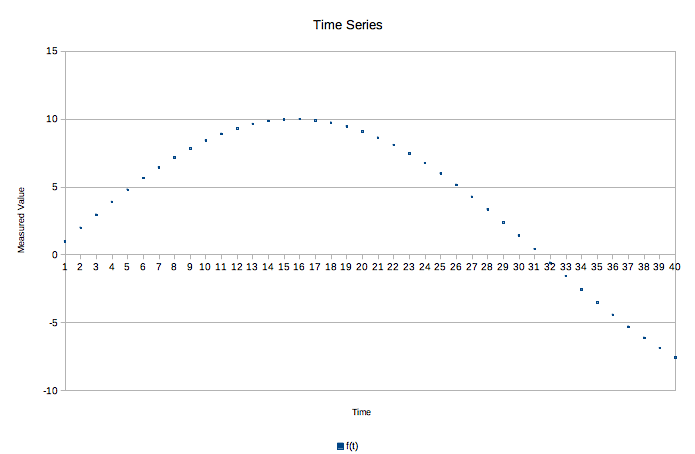
\includegraphics[width=0.8\linewidth]{fig0072.png}
  \caption{Времеви ред следващ синус функция}
\label{fig0072}
\end{figure}

\begin{figure}[H]
  \centering
  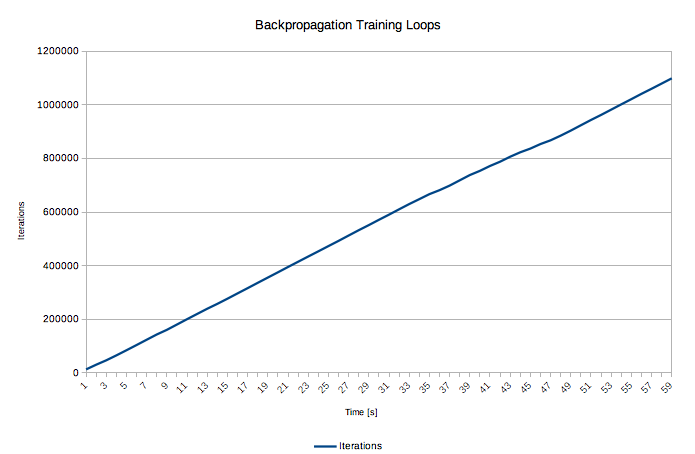
\includegraphics[width=0.8\linewidth]{fig0073.png}
  \caption{Backpropagation брой тренировъчни цикли}
\label{fig0073}
\end{figure}

\begin{figure}[H]
  \centering
  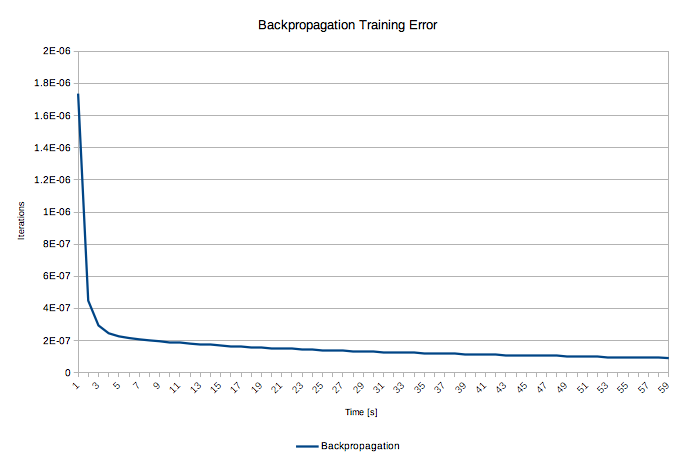
\includegraphics[width=0.8\linewidth]{fig0074.png}
  \caption{Backpropagation обща грешка на изкуствената невронна мрежа}
\label{fig0074}
\end{figure}

\begin{figure}[H]
  \centering
  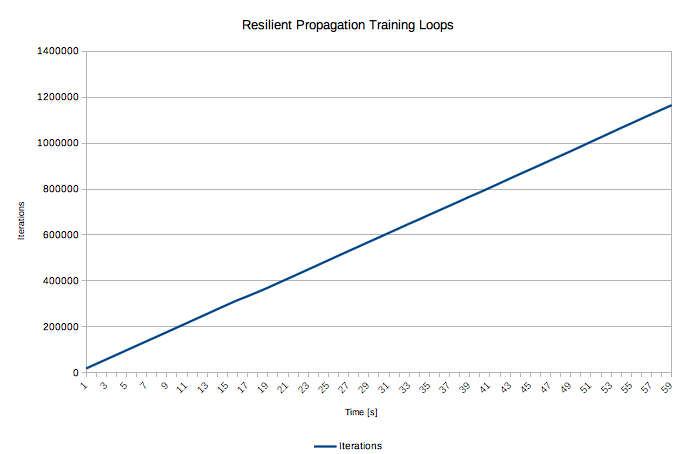
\includegraphics[width=0.8\linewidth]{fig0075.png}
  \caption{ResilientPropagation брой тренировъчни цикли}
\label{fig0075}
\end{figure}

\begin{figure}[H]
  \centering
  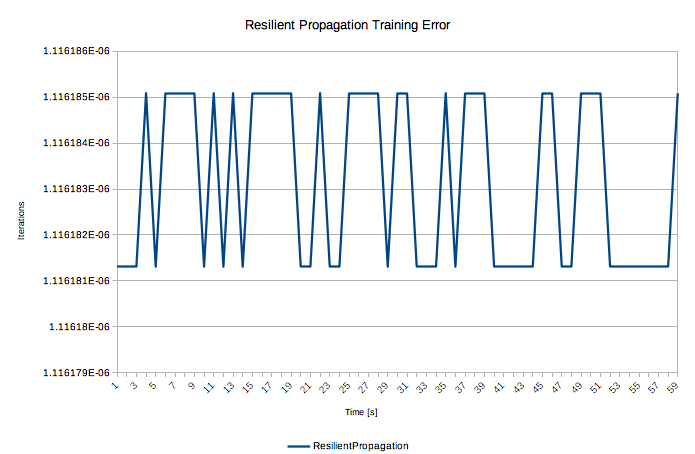
\includegraphics[width=0.8\linewidth]{fig0076.png}
  \caption{ResilientPropagation обща грешка на изкуствената невронна мрежа}
\label{fig0076}
\end{figure}

\begin{figure}[H]
  \centering
  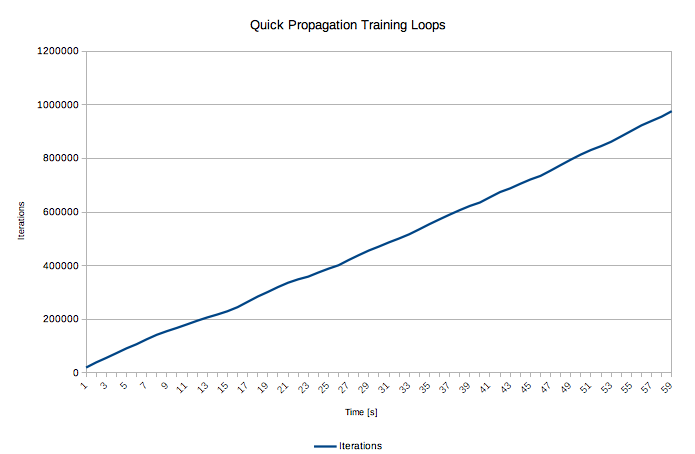
\includegraphics[width=0.8\linewidth]{fig0077.png}
  \caption{QuickPropagation брой тренировъчни цикли}
\label{fig0077}
\end{figure}

\begin{figure}[H]
  \centering
  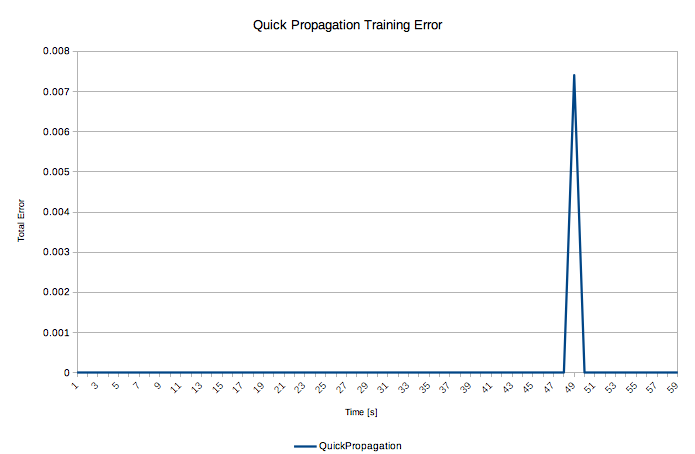
\includegraphics[width=0.8\linewidth]{fig0078.png}
  \caption{QuickPropagation обща грешка на изкуствената невронна мрежа}
\label{fig0078}
\end{figure}

\begin{figure}[H]
  \centering
  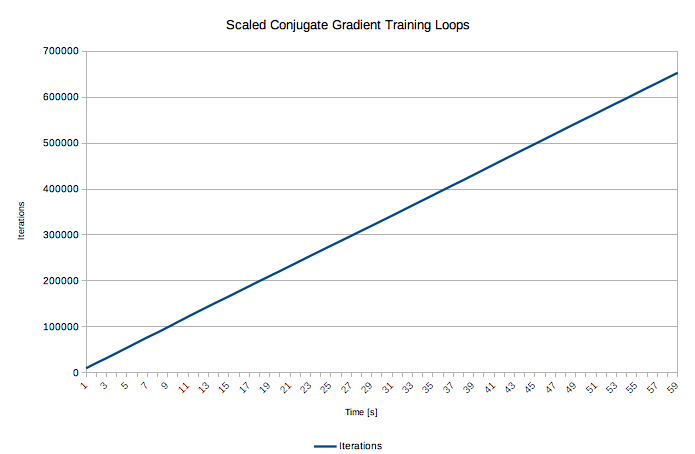
\includegraphics[width=0.8\linewidth]{fig0079.png}
  \caption{ScaledConjugateGradient брой тренировъчни цикли}
\label{fig0079}
\end{figure}

\begin{figure}[H]
  \centering
  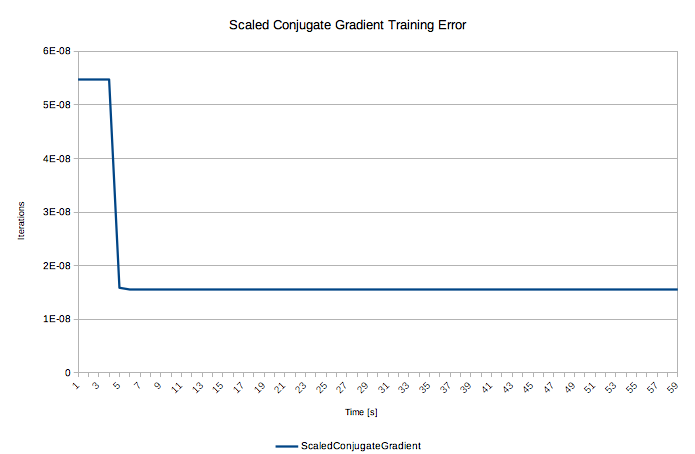
\includegraphics[width=0.8\linewidth]{fig0080.png}
  \caption{ScaledConjugateGradient обща грешка на изкуствената невронна мрежа}
\label{fig0080}
\end{figure}

\begin{figure}[H]
  \centering
  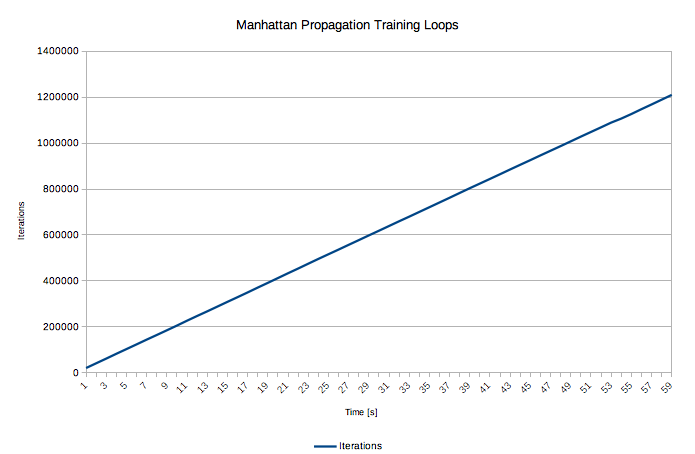
\includegraphics[width=0.8\linewidth]{fig0081.png}
  \caption{ManhattanPropagation брой тренировъчни цикли}
\label{fig0081}
\end{figure}

\begin{figure}[H]
  \centering
  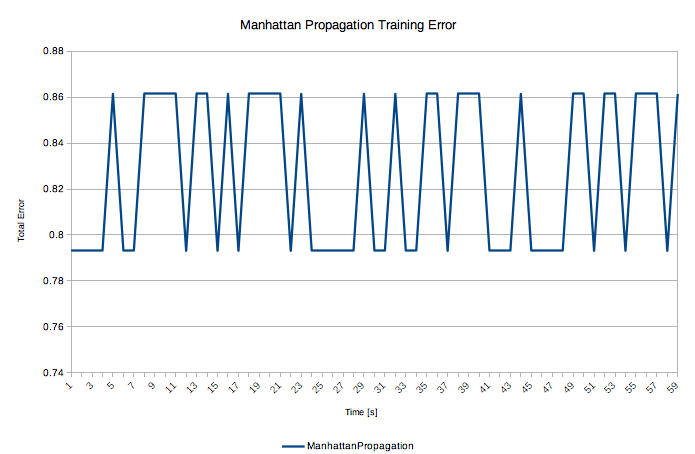
\includegraphics[width=0.8\linewidth]{fig0082.png}
  \caption{ManhattanPropagation обща грешка на изкуствената невронна мрежа}
\label{fig0082}
\end{figure}

\subsection{Цена на биткойн}

\begin{figure}[H]
  \centering
  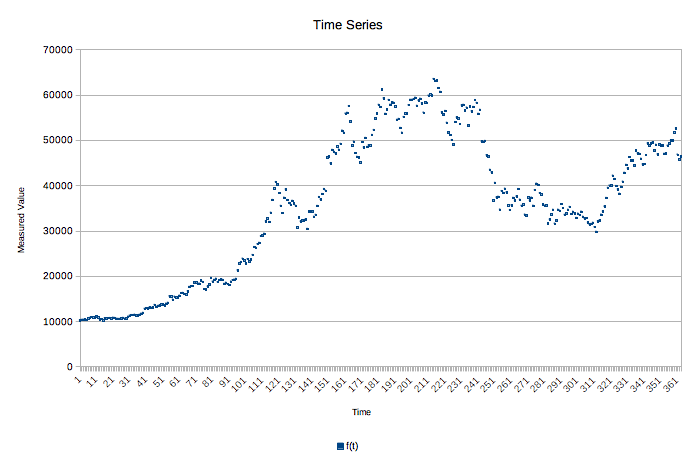
\includegraphics[width=0.8\linewidth]{fig0083.png}
  \caption{Времеви ред с цената на биткойн}
\label{fig0083}
\end{figure}

\begin{figure}[H]
  \centering
  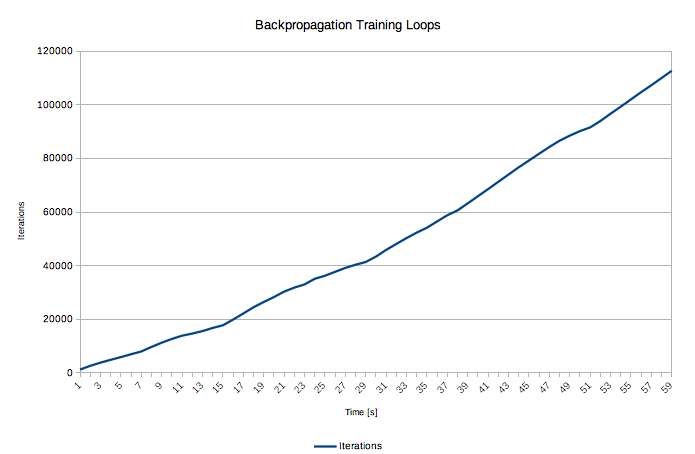
\includegraphics[width=0.8\linewidth]{fig0084.png}
  \caption{Backpropagation брой тренировъчни цикли}
\label{fig0084}
\end{figure}

\begin{figure}[H]
  \centering
  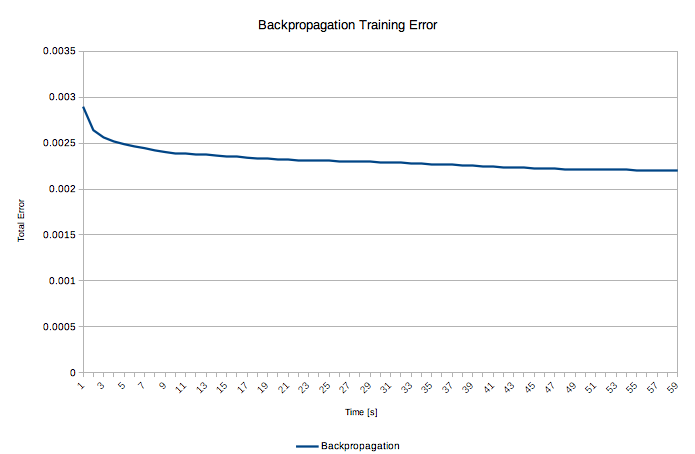
\includegraphics[width=0.8\linewidth]{fig0085.png}
  \caption{Backpropagation обща грешка на изкуствената невронна мрежа}
\label{fig0085}
\end{figure}

\begin{figure}[H]
  \centering
  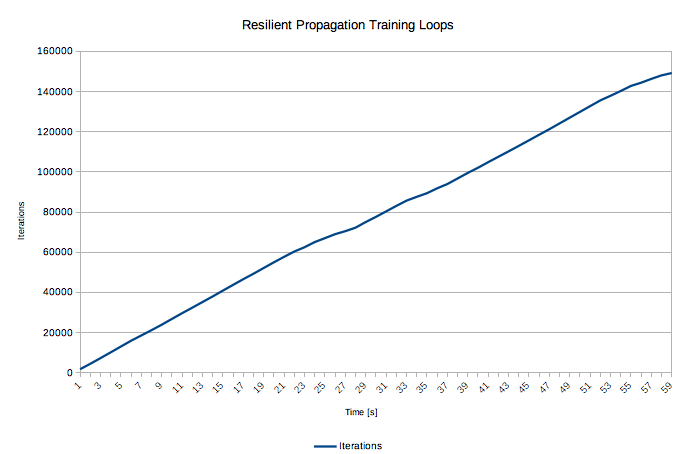
\includegraphics[width=0.8\linewidth]{fig0086.png}
  \caption{ResilientPropagation брой тренировъчни цикли}
\label{fig0086}
\end{figure}

\begin{figure}[H]
  \centering
  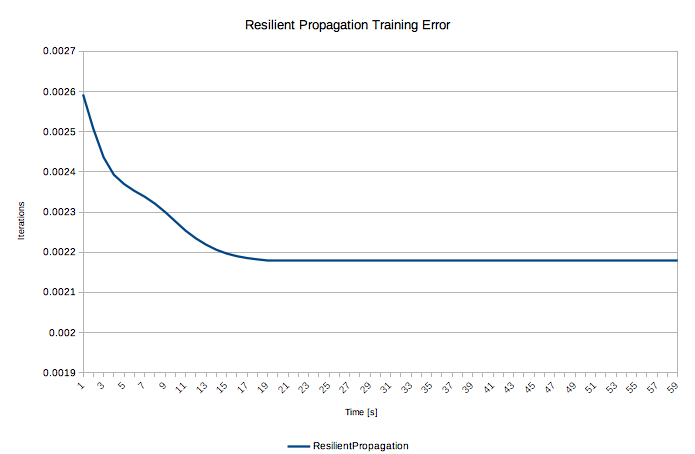
\includegraphics[width=0.8\linewidth]{fig0087.png}
  \caption{ResilientPropagation обща грешка на изкуствената невронна мрежа}
\label{fig0087}
\end{figure}

\begin{figure}[H]
  \centering
  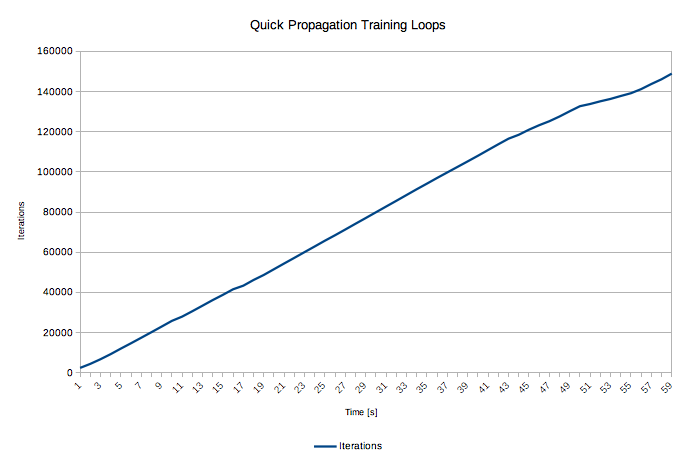
\includegraphics[width=0.8\linewidth]{fig0088.png}
  \caption{QuickPropagation брой тренировъчни цикли}
\label{fig0088}
\end{figure}

\begin{figure}[H]
  \centering
  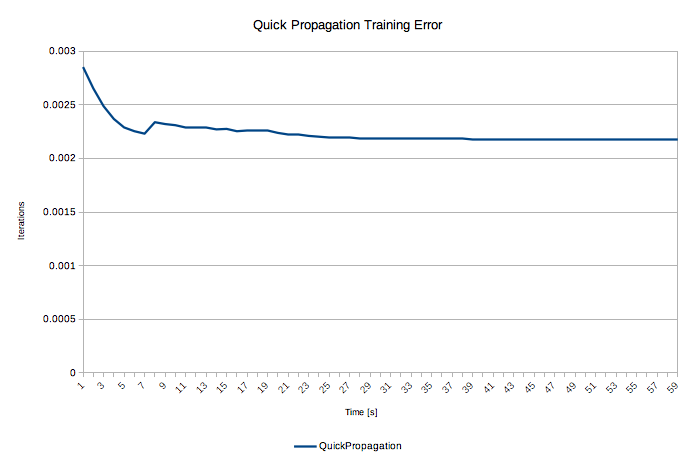
\includegraphics[width=0.8\linewidth]{fig0089.png}
  \caption{QuickPropagation обща грешка на изкуствената невронна мрежа}
\label{fig0089}
\end{figure}

\begin{figure}[H]
  \centering
  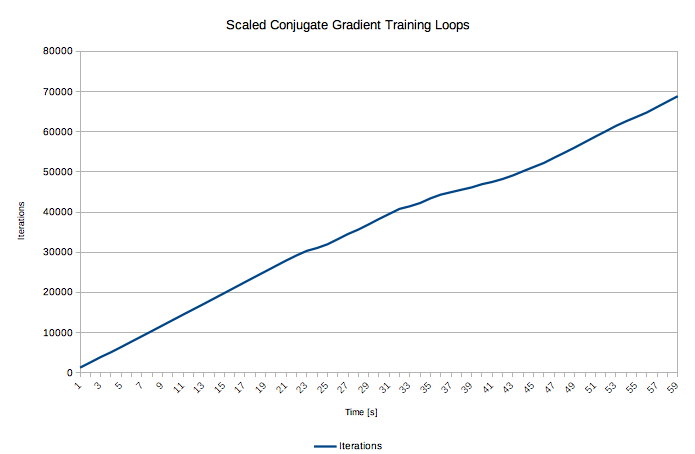
\includegraphics[width=0.8\linewidth]{fig0090.png}
  \caption{ScaledConjugateGradient брой тренировъчни цикли}
\label{fig0090}
\end{figure}

\begin{figure}[H]
  \centering
  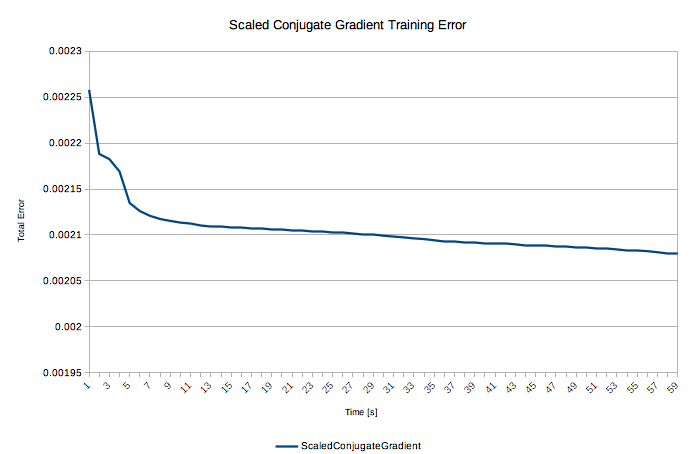
\includegraphics[width=0.8\linewidth]{fig0091.png}
  \caption{ScaledConjugateGradient обща грешка на изкуствената невронна мрежа}
\label{fig0091}
\end{figure}

\begin{figure}[H]
  \centering
  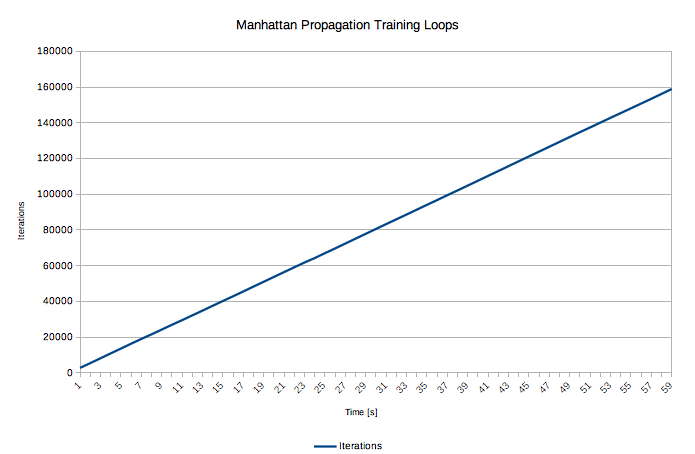
\includegraphics[width=0.8\linewidth]{fig0092.png}
  \caption{ManhattanPropagation брой тренировъчни цикли}
\label{fig0092}
\end{figure}

\begin{figure}[H]
  \centering
  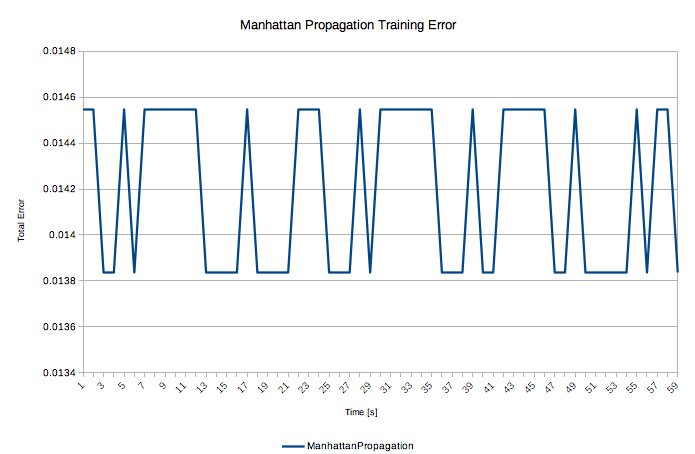
\includegraphics[width=0.8\linewidth]{fig0093.png}
  \caption{ManhattanPropagation обща грешка на изкуствената невронна мрежа}
\label{fig0093}
\end{figure}

\subsection{Анализ на ефективността}

Резултатите (Фиг. \ref{fig0073}-\ref{fig0082}) от проведените експерименти показват, че класическият алгоритъм с обратно разпространение на грешката се представя най-добре, за времеви ред с относително опростена структура. Резултатите (Фиг. \ref{fig0084}-\ref{fig0093}) от експериментите показват, че при времеви ред със значително по-сложна структура, еластичното (Resilient) обучение е с най-добра ефективност. И при двата комплекта данни, Манхатън обучението показва най-слаба ефективност. 

\begin{lstlisting}[caption=Случаен избор на точните числени методи, language=Java, basicstyle=\tiny, label=list0023]
propagation = propagations[PRNG.nextInt(propagations.length)];
\end{lstlisting}

Макар и някои от използваните алгоритми за обучение да не дават твърде голяма ефективност, те дават допълнително разнообразие в генетичния фонд на еволюционните алгоритми, които са в хибридна употреба с точните числени алгоритми. Всеки от петте точни числени алгоритъма бива избиран на случаен принцип, равно вероятно, за участие в обучението (Листинг \ref{list0021} и \ref{list0023}). Обучението на изкуствената невронна мрежа не започва от случайно подбрани тегла, а продължава от там до където е стигнато при предишна обучаваща сесия. 

